\documentclass[a4paper]{article}
\usepackage[a4paper]{geometry}
\usepackage{amsmath}
\usepackage{amsfonts}
\usepackage{amssymb}
\usepackage{float}
\usepackage{graphicx}
\graphicspath{{./images/}}
\begin{document}
	\begin{center}
		\textbf{\LARGE Assignment 10}\linebreak\linebreak
		{\large AVIK BANERJEE (3374885), SOUMYADEEP BHATTACHARJEE (3375428)}
	\end{center}
\section*{Exercise 10.1}
\begin{enumerate}
	\item[a)] An R script to generate 10000 random samples from a normal distribution around 6 with standard deviation 1.5:
	\begin{verbatim}
	> a <- rnorm(n=10000,mean=6,sd=1.5)
	\end{verbatim}
	\item[b)] An R script to generate 500 random samples from a bimodal distribution with modes 4 and 7 is:
	\begin{verbatim}
	> x <- rnorm(n=1000,mean=4,sd=0.5)
	> y <- rnorm(n=1000,mean=7,sd=0.5)
	> z <- cbind(x,y)
	> z <- sample(z,500)
	\end{verbatim}
	\item[c)] Histogram of sample data in part (a):
	\begin{figure}[H]
		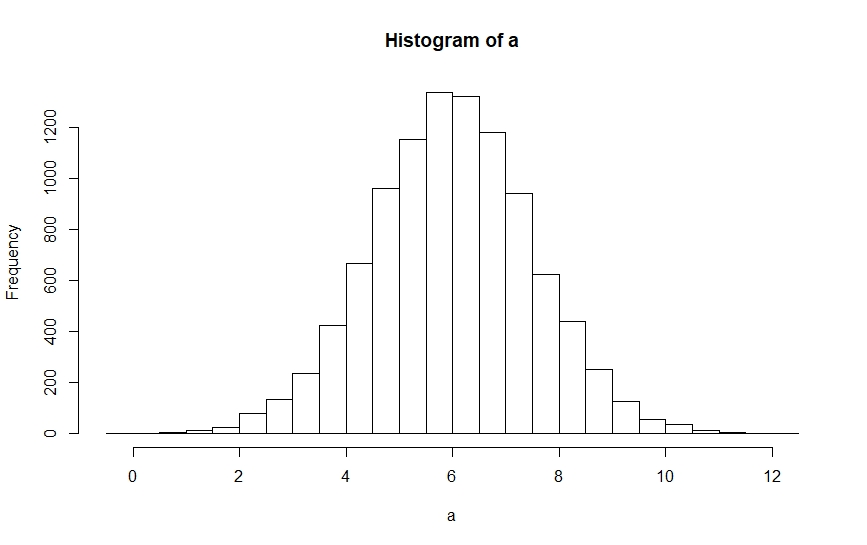
\includegraphics[width=\linewidth]{hist_1.jpeg}
	\end{figure}
	Histogram of sample data in part (b):
	\begin{figure}[H]
		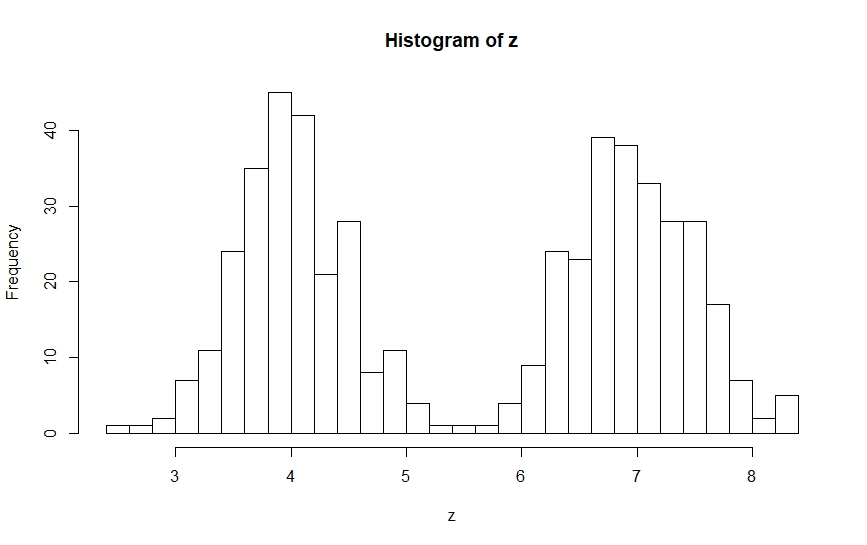
\includegraphics[width=\linewidth]{hist_2.jpeg}
	\end{figure}
	\item[d)] The description in the question does not suggest a good controlled experiment as it does not say anything about other factors that may affect the attack of pests on the crops, such as the type of crop used, types of manure used, characteristics of the soil and so on.
	\paragraph{}This experiment can be improved by ensuring the same crops are used on both the fields with the same soil characteristics, similar usage of manure, similar environmental conditions such as exposure to sunlight and others, and then applying pesticide to one field and testing the effects. Another approach may include using the same field, carefully dividing the crops into two groups, one of which is exposed to pesticides, while the other is not, and then testing the effects on the two groups.
\end{enumerate}
\section*{Exercise 10.2}
Given the sample values
\begin{equation*}
S=\{1,4,2,6,4,7,3,4,2,5,39,0,5,8,-3,1,5,4,2\}
\end{equation*}
For ease of calculation, we can sort the values
\begin{equation*}
S=\{-3,0,1,1,2,2,2,3,4,4,4,4,5,5,5,6,7,8,39\}
\end{equation*}
\begin{enumerate}
	\item[a)] The mode is the most frequently occuring value. The mode in this case is \textbf{4}.
	\item[b)] The median value: 
	\begin{equation*}
	x_{\frac{N+1}{2}}=x_{\frac{20}{2}}=x_{10}=\mathbf{4}
	\end{equation*}
	\item[c)] The mean is
	\begin{equation*}
	\bar{x}=\frac{1}{n}\sum_{i=1}^{n}x_i=\frac{\sum_{i=1}^{19}x_i}{19}=\frac{99}{19}=\mathbf{5.2105}
	\end{equation*}
	\item[d)] The sum of squared errors (SSE) is
	\begin{equation*}
	\sum_{i=1}^{n}(x_i-\bar{x})^2 = \sum_{i=1}^{19}(x_i-5.2105)^2 = \mathbf{1325.15}
	\end{equation*}
	\item[e)] Variance 
	\begin{equation*}
	\sigma^2=\frac{\text{SSE}}{n-1} = \frac{1325.15}{19-1} = \mathbf{73.61}
	\end{equation*}
	\item[f)] Standard Deviation:
	\begin{equation*}
	\sigma=\sqrt{\text{Variance}} = \sqrt{73.61} = \mathbf{8.58}
	\end{equation*}
	\item[f)] Standard Error:
	\begin{equation*}
	\text{SE}=\frac{\sigma}{\sqrt{n}} = \frac{8.58}{\sqrt{19}} = \mathbf{1.96}
	\end{equation*}
	\item[h)] 90\% Confidence interval
	\begin{equation*}
	\text{CI}_{0.90} = \bar{x} \pm 1.645*\text{SE} = 5.2105 \pm 3.2242 = \mathbf{[1.9863,8.4347]}
	\end{equation*}
\end{enumerate}
\section*{Exercise 10.3}
\begin{enumerate}
	\item[a)] Two reasons why samples from two groups can have very different means:
	\begin{itemize}
		\item The difference could be a result of the conditions being tested. One of the groups may be a control group and the treatment being applied on the experimental group changes its mean.
		\item The difference could appear purely by chance from the intrinsic characteristics of the group participants that are skewed in one group due to lack of randomization in group allocation.
	\end{itemize}
	\item[b)] The threshold probability used to reject the null hypothesis is 5\%, that is, if the p-value is lower than 5\%, we have statistically significant results, as the probability that we are incorrectly rejecting the null hypothesis is lower than the threshold set by Fisher, 5\%.
	\item[c)] We can conclude the following from a p-value below 0.05:
	\begin{enumerate}
		\item[1.] The result is statistically significant.
		\item[8.] We can reject $H_0$.
	\end{enumerate}
\item[d)] Significance testing can sometimes be misleading due to the influence of sample sizes. Statistically significant results do not always imply an important effect. When using large samples, trivial results may also be rendered statistically significant. To avoid this, effect sizes need to be reported. Effect sizes denote the importance of an effect through standardized measures of the magnitude of an effect. 
\item[e)] \textbf{Cohen's d} and \textbf{Pearson's r} are two common measures for effect sizes.
\item[f)] \begin{itemize}
	\item A priori power analysis can be used to estimate the optimum sample size for the study.
	\item Power analysis can be used to perform sensitivity analysis to estimate the effect size.
\end{itemize}
\end{enumerate}
\section*{Exercise 10.4}
\begin{enumerate}
	\item[a)] The Kolmogorov-Smirnov test is less sensitive to small n and is less strict than the Shapiro-Wilk test. Hence the Shapiro-Wilk test will be preferred for small number of samples.
	\item[b)] To ensure normality, the data can be visualised using Histograms and Q-Q plots. 
\end{enumerate}
\end{document}